\section{201604-1 折点计数}

\subsection{题目描述}%题目描述请保留在文档内

给定$n$个整数表示一个商店连续$n$天的销售量。如果某天之前销售量在增长,而后一天销售量减少,则称这一天为折点,反过来如果之前销售量减少而后一天销售量增长,也称这一天为折点。其他的天都不是折点。如图\ref{fig:201604-1-1}中,第3天和第6天是折点。

\begin{figure}[H]
    \centering
    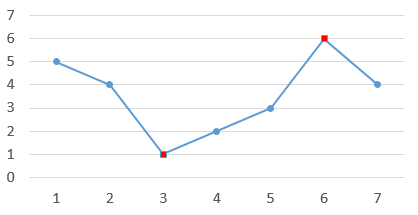
\includegraphics{chapter3/exam201604_1/p1.png}
    \caption{折点示意图}
    \label{fig:201604-1-1}
\end{figure}

给定$n$个整数$a_1,a_2,\cdots,a_n$表示销售量,请计算出这些天总共有多少个折点。

为了减少歧义,我们给定的数据保证:在这$n$天中相邻两天的销售量总是不同的,即$a_{i-1} \neq a_i$。注意,如果两天不相邻,销售量可能相同。

\subsection{输入格式}

输入的第一行包含一个整数$n$。

第二行包含$n$个整数,用空格分隔,分别表示$a_1,a_2,\cdots,a_n$。

\subsection{输出格式}

输出一个整数,表示折点出现的数量。

\subsection{样例输入}

\begin{lstlisting}[numbers=none]
7
5 4 1 2 3 6 4
\end{lstlisting}

\subsection{样例输出}

\begin{lstlisting}[numbers=none]
2
\end{lstlisting}

\subsection{评测用例规模与约定}

所有评测用例满足:$1\leq n\leq1000$,每天的销售量是不超过10000的非负整数。

\subsection{对讲义中代码的点评或纠错}
清晰简单: 代码结构相对简单,易于理解。它有一个主循环,用于逐个读取输入的整数,并在每次迭代中检查条件。\\
\indent
使用了有意义的变量名: 变量名命名得相对清晰,例如,n用于存储整数的数量,pre和cur用于存储前一个和当前的整数,cnt用于计数满足条件的数字对。\\
\indent 
条件判断简单明了: 条件判断语句 (pre < cur \&\& cur > next) || (pre > cur \&\& cur < next) 是简单明了的,容易理解。
\subsection{自己原创的代码的点评与注释}

首先读取整数 n,表示销售量的天数。然后,读取包含 n 个整数的数组,表示每天的销售量。接下来,程序遍历销售量数组,检查每一天是否为折点,并计算折点的数量。最后,输出折点的数量。

\begin{lstlisting}[language=C++]
    #include <iostream>
    using namespace std;
    
    int main() {
        // 读取输入
        int n;
        cin >> n;
    
        // 读取销售量数组
        int sales[n];
        for (int i = 0; i < n; ++i) {
            cin >> sales[i];
        }
    
        // 计算折点数量
        int count = 0;
        for (int i = 1; i < n - 1; ++i) {
            if ((sales[i] > sales[i - 1] && sales[i] > sales[i + 1]) ||
                (sales[i] < sales[i - 1] && sales[i] < sales[i + 1])) {
                count++;
            }
        }
    
        // 输出结果
        cout << count << endl;
    
        return 0;
    }        
\end{lstlisting}